\section{Motivation}
% R at google https://web.archive.org/web/20150125042733/https://plus.google.com/+ResearchatGoogle/posts/em2i7TEpHgj
% IF: https://jcr.clarivate.com/jcr-jp/journal-profile?journal=R%20J&year=2021&fromPage=%2Fjcr%2Fbrowse-journals
% 3.084 / 1.68
% TODO: neue DAten sind schwer zu kriegen/unmöglich > 2 Mio downloads des R basispakets im letzten Monat
% Linked in ~3000 R Programmging language jobs
\begin{frame}{Usage of R}
\vspace*{-8mm}\centering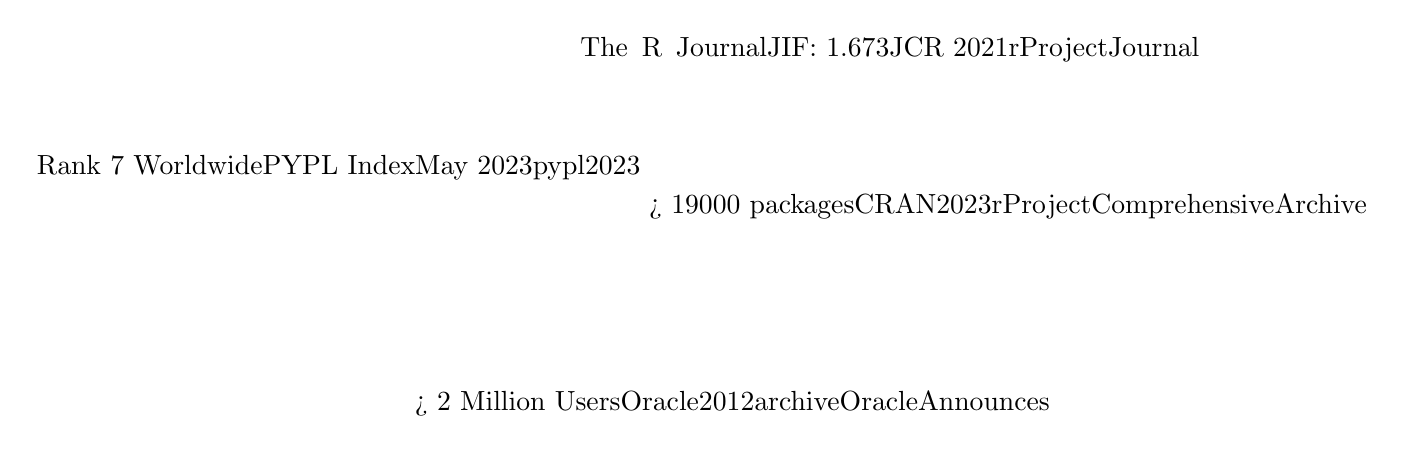
\begin{tikzpicture}% [overlay, remember picture]
   \onslide<2->{\node at (0,0) {\typesetBox{Rank 7 Worldwide}{PYPL Index}{May 2023}{pypl2023}};}
   \onslide<3->{\node at (7,1.5) {\typesetBox{\say{The\, R\, Journal}}{JIF: \num{1.673}}{JCR~2021}{rProjectJournal}};}
   \onslide<4->{\node at (5,-3) {\typesetBox{>~2 Million Users}{Oracle}{2012}{archiveOracleAnnounces}};}
   \onslide<5->{\node at (8.5,-.5) {\typesetBox{>~\num{19000} packages}{CRAN}{2023}{rProjectComprehensiveArchive}};}
\end{tikzpicture}
\begin{tikzpicture}[@O]
   \node[FCite] at(current page.south west) {%
      \only<2->{\cite{pypl2023} \link{https://pypl.github.io/PYPL.html}{https://pypl.github.io/}}%
      \only<3->{\\\cite{rProjectJournal} \link{https://journal.r-project.org/}{https://journal.r-project.org/}}%
      \only<4->{\\\cite{archiveOracleAnnounces} \link{https://web.archive.org/web/20120211034626/https://www.oracle.com/us/corporate/press/1515738}{https://www.oracle.com/us/corporate/press/1515738 [archived]}}
      \only<5->{\\\cite{rProjectComprehensiveArchive} \link{https://cran.r-project.org/}{https://cran.r-project.org/}}
   };
\end{tikzpicture}\note[itemize]{%
\item Rang 7 in PYPL (PopularitY of Programming Language) mit 4.34\%, hinter PHP mit 5.5\%; vor TypeScript mit 2.88\%. Top: Python mit 27.27\%
\item Rang 16 in TIOBE mit 0.82\%
\item Eigenes Journal mit JIF (Journal Impact Factor) von 1.673 (2021); 2020 noch 3.984 (weitere Konferenzen wie useR! auch 2023)
\item Viele Nutzer: Oracle 2012 sagt mehr als 2 Millionen (mehr als 2 Mio Downloads des base Paket im letzten Monat).
\item Viel mehr: Google spricht von "sehr großer Code-Base" (mehr als 500 aktive Nutzer UserR! 2012) % https://blog.revolutionanalytics.com/2012/06/user-2012-highlights.html
}(2)%
\end{frame}
\addtocategory{@hide}{pypl2023,rProjectJournal,archiveOracleAnnounces,rProjectComprehensiveArchive}

\def\LinkMark#1{\textcolor{gray}{\scriptsize#1}}
%\def\Rect#1#2{\draw[rounded corners,gray] ([shift={(-.5mm,.5mm)}]#1.north west) rectangle ([shift={(.5mm,-.5mm)}]#2.south east);}
\newcommand\BraceRight[4][2mm]{\draw[line cap=round, gray,decorate,decoration={brace}] ([shift={(#1,.5mm)}]#2.north west-|#3.east) to[edge node={node[right=1mm,font=\small,align=left] {#4}}] ([shift={(#1,-.5mm)}]#3.south east);}
\newcommand\BraceBelow[4][.5mm]{\draw[line cap=round, gray,decorate,decoration={brace,mirror}] ([shift={(-.5mm,-#1)}]#2.south west) to[edge node={node[below=1mm,font=\small] {#4}}] ([shift={(.5mm,-#1)}]#3.south east);}
\def\Arrow#1#2{\draw[Kite-,line cap=round,gray,font=\small] ([xshift=2mm]#1.east) -- ++(5mm,0) node[right=1mm] {#2};}
\def\Out#1{{\color{lightgray}\sout{#1}}}

\begin{frame}[t]{Existing (Analysis) Support for R}
   \vspace*{-3mm}\begin{itemize}
      \itemsep10pt
      \item<2-> %\raisebox{-.248\height}{\includegraphics[height=1.5\baselineskip]{logos/RStudio-Logo-flat.pdf}}
      RStudio IDE\textsuperscript{\color{gray}\cite{RStudio}}\quad \LinkMark{\link{https://posit.co/products/open-source/rstudio/}{posit.co}}
      \begin{itemize}
         \item<3-> \Snode{rstudio-start}Syntax-highlighting and auto-completion
         \item<3-> Simple debugger
         \item<3-> \only<11-|handout:2>{\expandafter\Out}{Refactorings (rename, extract functions and variables)}\Snode{rstudio-end}
      \end{itemize}
      \item<4-> R~language~server\quad \LinkMark{\link{https://github.com/REditorSupport/languageserver/}{github.com/REditorSupport}}\begin{itemize}
         \item<5-> Syntax-highlighting and auto-completion
         \item<5-> \Snode{r-lang-start}\only<12-|handout:2>{\expandafter\Out}{Reference tracing} % (wrong, uses XPath-Expressions)
         \item<5-> \only<12-|handout:2>{\expandafter\Out}{Refactorings (rename)}\Snode{r-lang-end} % (uses XPath-Expressions)
      \end{itemize}
\end{itemize}\vspace*{-\topsep}%
\begin{columns}[onlytextwidth,t]
\column{.4\linewidth}
\begin{itemize}[<+(1)->]
   \item<6-> \T{\{}lintr\T{\}}\quad \LinkMark{\link{https://github.com/r-lib/lintr}{github.com/r-lib/lintr}} \begin{itemize}
      \item<7-> Style checker
      \item<7-> Syntax errors
      \item<7-> \Snode{lintr-start}\only<13-|handout:2>{\expandafter\Out}{Potential semantic errors}\Snode{lintr-end}
   \end{itemize}
\end{itemize}
\column{.6\linewidth}
\begin{itemize}[<+(1)->]
   \item<8-> CodeDepends\textsuperscript{\color{gray}\cite{lang_codedepends_2018}}\quad \LinkMark{\link{https://github.com/duncantl/CodeDepends}{github.com/duncantl/CodeDepends}} \begin{itemize}
      \item<9-> \only<14-|handout:2>{\expandafter\Out}{Dependency analysis}\Snode{dep-analysis}
      \item<9-> Creation of call-graphs
      \item<9-> \only<15-|handout:2>{\expandafter\Out}{Classification of tasks}\Snode{classification}
   \end{itemize}
\end{itemize}
\begin{tikzpicture}[@O]
   % xshift=-6mm, | -|current page.east
   % \draw[rounded corners] ([shift={(-.5mm,.5mm)}]rstudio-start.north west) rectangle ([shift={(.5mm,-.5mm)}]rstudio-end.south east);
   % \BraceRight{rstudio-start}{rstudio-end}{}
   \onslide<10-|handout:2>{\Arrow{rstudio-end}{Often wrong (simple heuristics)}}
   \onslide<12-|handout:2>{
      \BraceRight[3.1cm]{r-lang-start}{r-lang-end}{Often wrong\\Based on XPath-expressions}
   }
   \onslide<13-|handout:2>{
      \BraceBelow{lintr-start}{lintr-end}{XPath-expressions, packages}
   }
   \onslide<14-|handout:2>{
      \Arrow{dep-analysis}{Only top scope}
   }
   \onslide<15-|handout:2>{
      \Arrow{classification}{Regex-based matching}
   }
\end{tikzpicture}
\end{columns}
\note[itemize]{%
\item RStudio von posit (hauptsächlich in Java/C++)
\item TODO: es gibt auch andere kleinere wie reformatter, rclean, ... optimizer rco...
}(4)%
   % optimizr, tidyverse, RDocumentation, CodeDepends/CodeTools, R language server
\end{frame}
\addtocategory{@hide}{RStudio}